\documentclass{article}
\usepackage[utf8]{inputenc}
\usepackage{subfiles} 
\usepackage{fancyhdr}
\usepackage{graphicx}

\title{DevOps projectreport \\[2ex] 
\includegraphics[scale=0.1]{images/ITU_logo_UK.jpg}}
\author{Joachim Køcher Kelsen (jokk@itu.dk) \and Victor Nordestgaard (vino@itu.dk) \and Isabella Drest Rasmussen (iras@itu.dk) \and Anne Siemkowicz (asie@itu.dk) \and Bjørnar Haugstad Jåtten(bjja@itu.dk)}
\date{19 May 2021}

\usepackage{geometry}
\geometry{
 a4paper,
 total={210mm,297mm},
 left=30mm,
 right=30mm,
 top=25mm,
 bottom=20mm,
 }

\pagestyle{fancy}
\fancyhf{}
\rhead{Pythonkindergarten/Group J}
\lhead{DevOps projectreport}
\rfoot{Page \thepage}

\begin{document}{}

\maketitle

\newpage

\tableofcontents

\newpage

\subfile{sections/introduction.tex}

\newpage

\subfile{sections/LessonsLearnedPerspective.tex}

\newpage

\subfile{sections/ProcessPerspective.tex}

\newpage

\subfile{sections/SystemsPerspective.tex}

\newpage

\section{References}

\begin{thebibliography}{9}
\bibitem{devopshandbook} 
Gene Kim.
\textit{The DevOps Handbook: How to Create World-Class Agility, Reliability, and Security in Technology Organizations}. 
2016

\bibitem{lecture02} 
Helge Pfeiffer. 
\textit{Session 02: Version control systems (Git), branching strategies, and collaborative development workflows}. 

\bibitem{prometheusnet} 
https://github.com/prometheus-net/prometheus-net

\bibitem{prometheusdotnetmetrics} 
https://github.com/djluck/prometheus-net.DotNetRuntime

\bibitem{prometheusaspnet} 
https://github.com/rocklan/prometheus-net.AspNet

\end{thebibliography}

\newpage

\section{Appendix}
\begin{figure}[h!]
    \centering
    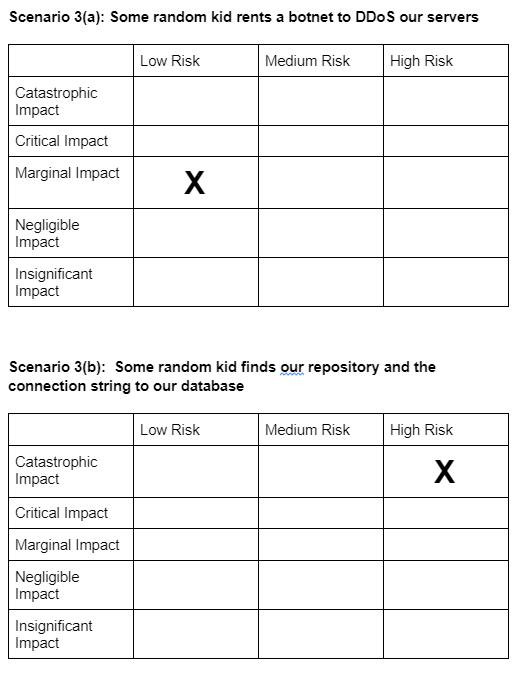
\includegraphics[scale=0.5]{images/risk_1.PNG}
    \caption{ Scenario 3a and 3b }
\end{figure}

\begin{figure}[h!]
    \centering
    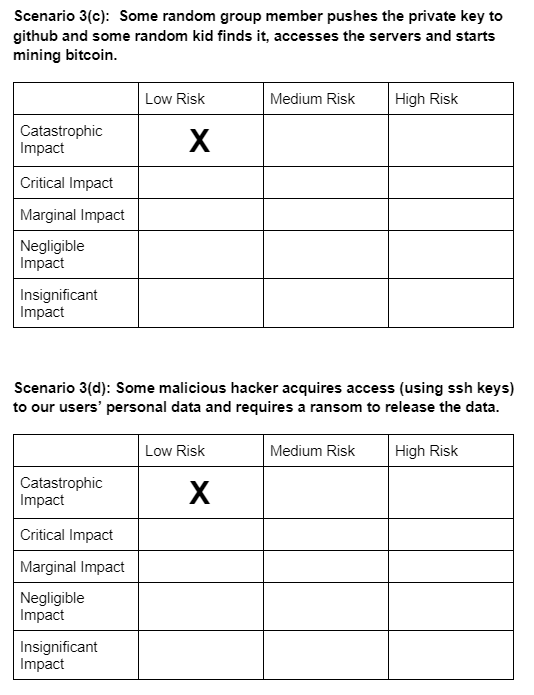
\includegraphics[scale=0.5]{images/risk_2.PNG}
    \caption{ Scenario 3c and 3d }
\end{figure}

\begin{figure}[h!]
    \centering
    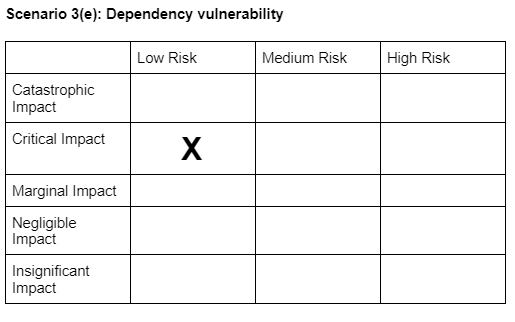
\includegraphics[scale=0.5]{images/risk_3.PNG}
    \caption{ Scenario 3e }
\end{figure}

\begin{figure}[h!]
    \centering
    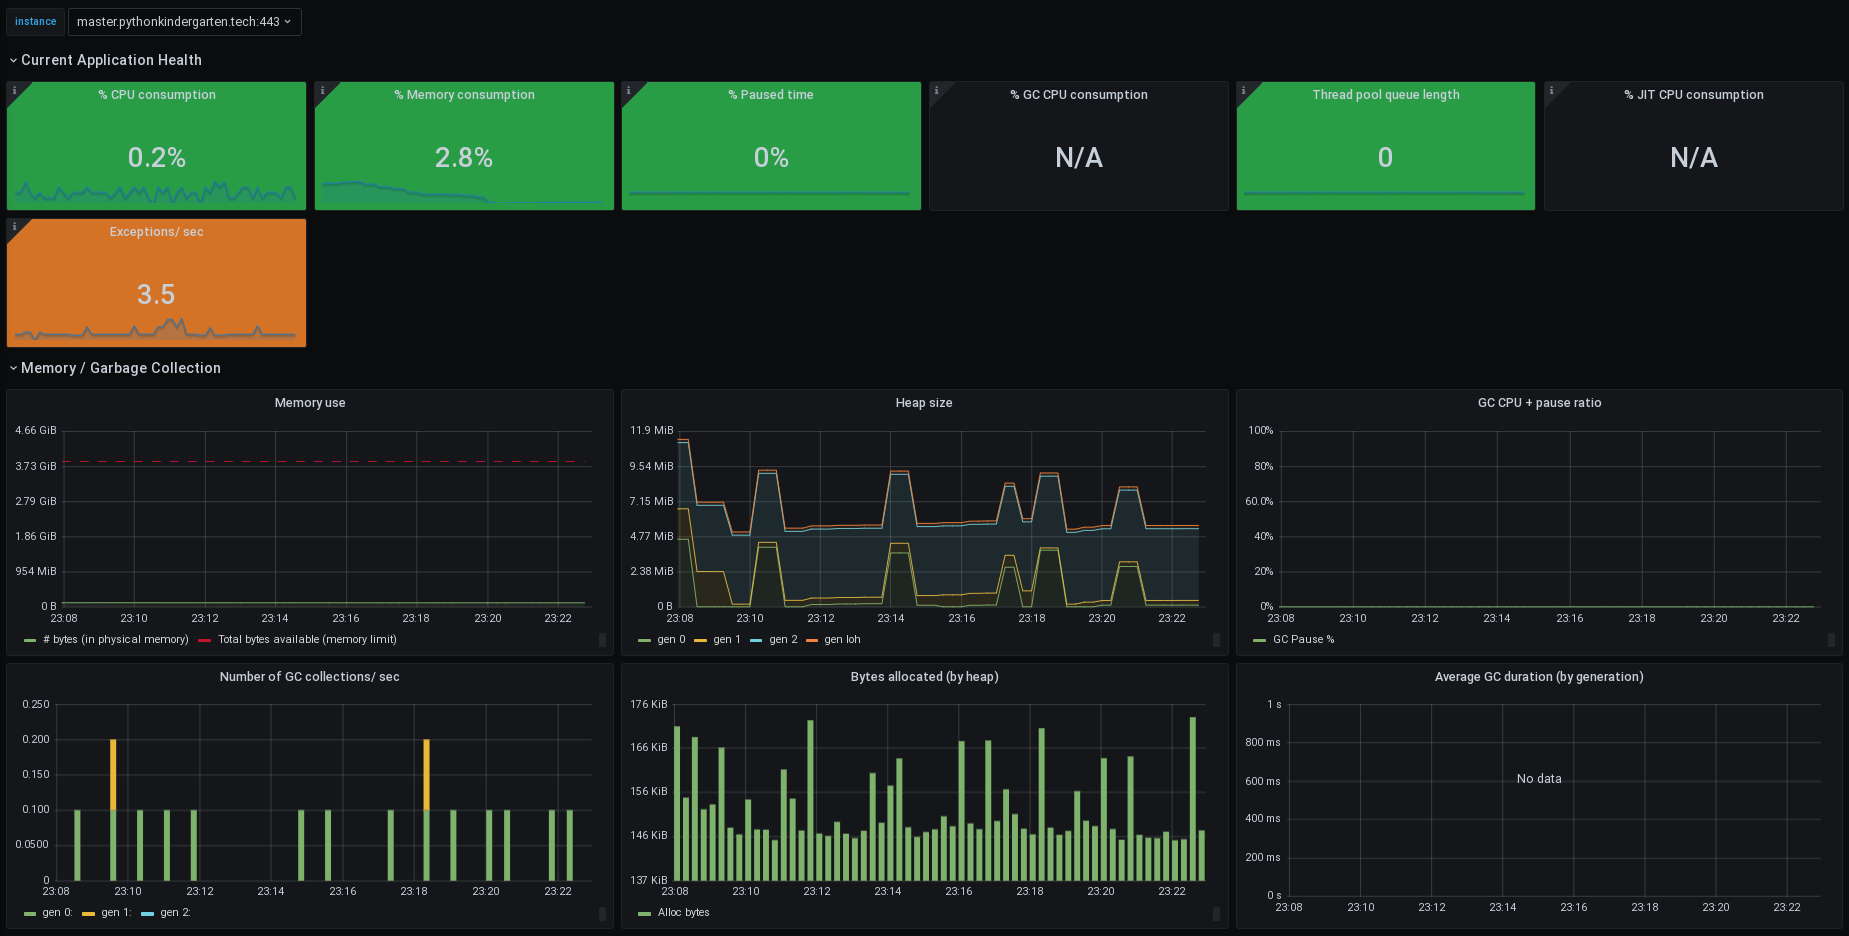
\includegraphics[scale=0.2]{images/grafana_1.png}
    \caption{ Our graphs in Grafana }
\end{figure}

\begin{figure}[h!]
    \centering
    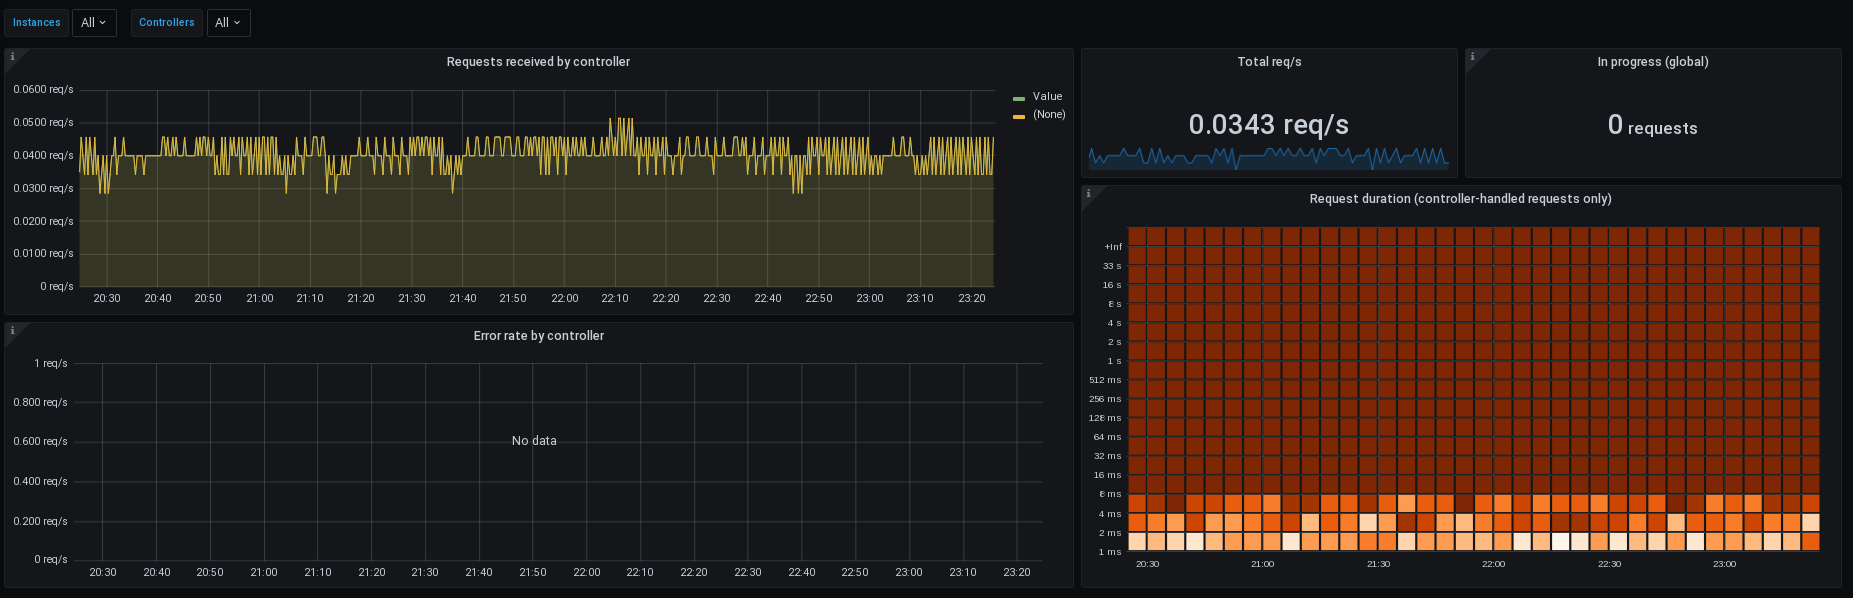
\includegraphics[scale=0.2]{images/grafana_2.png}
    \caption{ Our graphs in Grafana }
\end{figure}

\begin{figure}[h!]
    \centering
    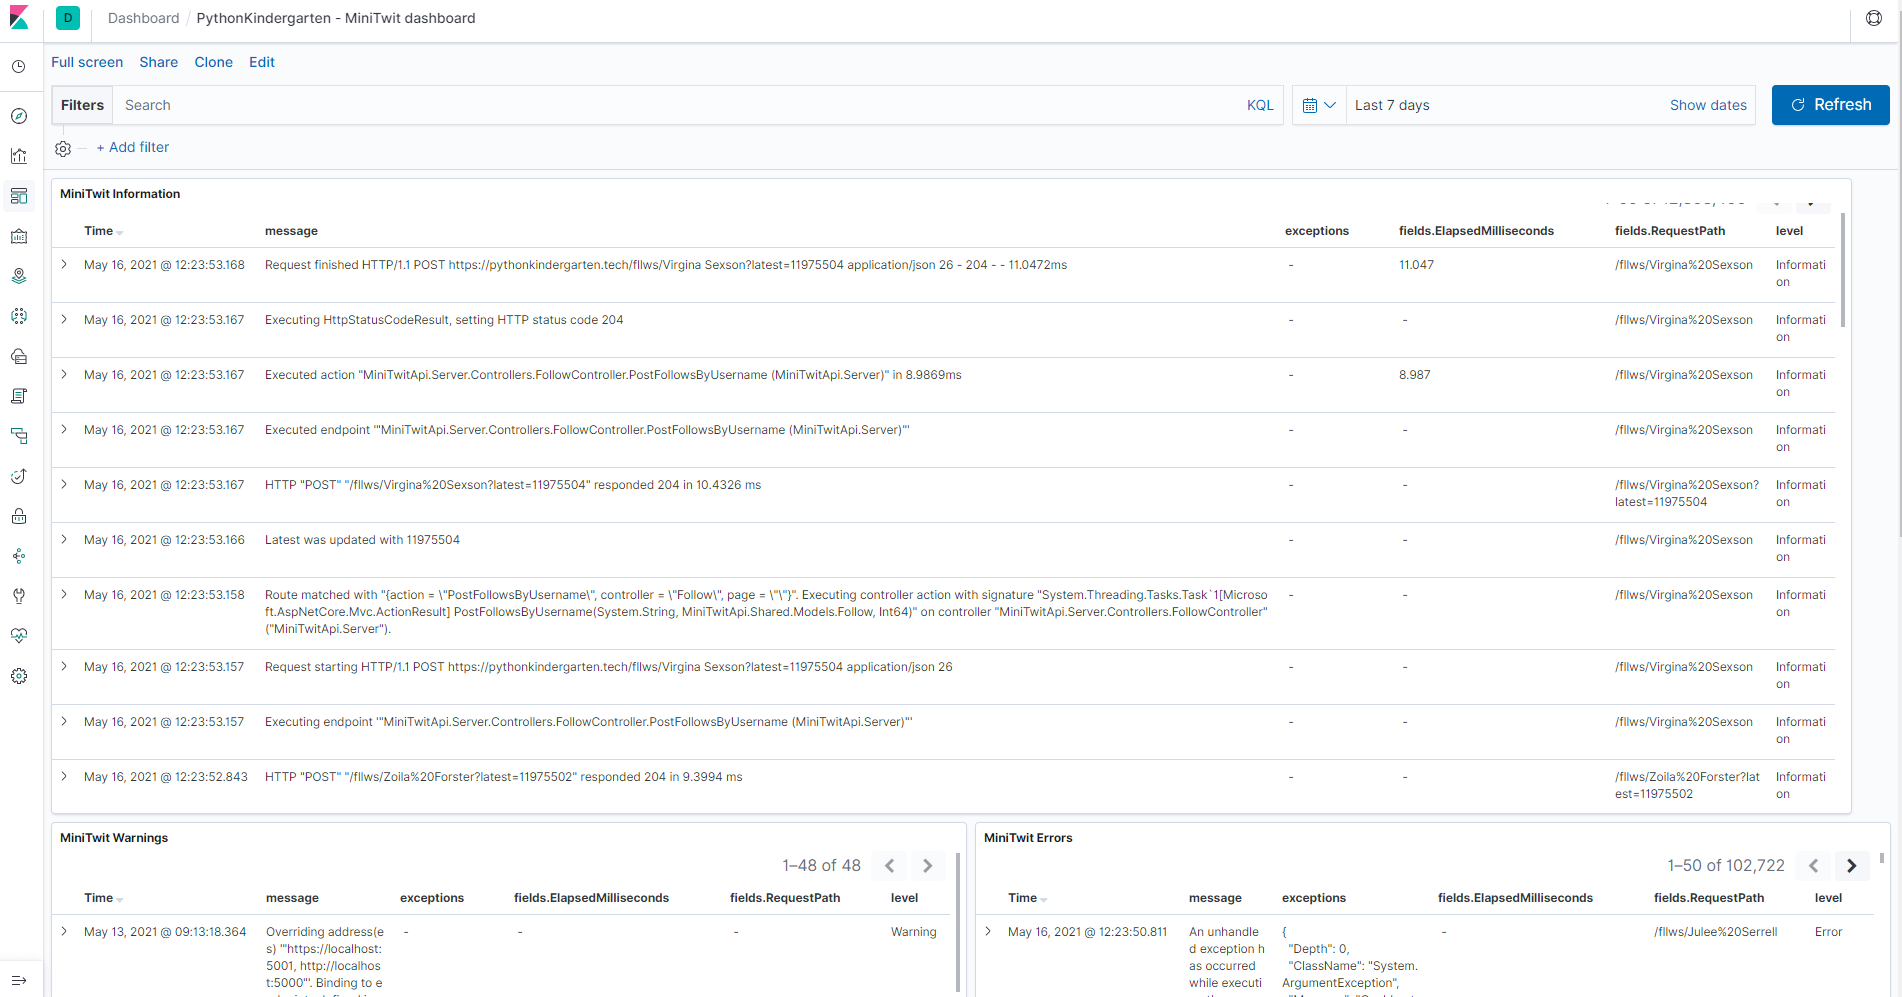
\includegraphics[scale=0.2]{images/kibana_1.png}
    \caption{ Current setup in Kibana }
\end{figure}

\begin{figure}[h!]
    \centering
    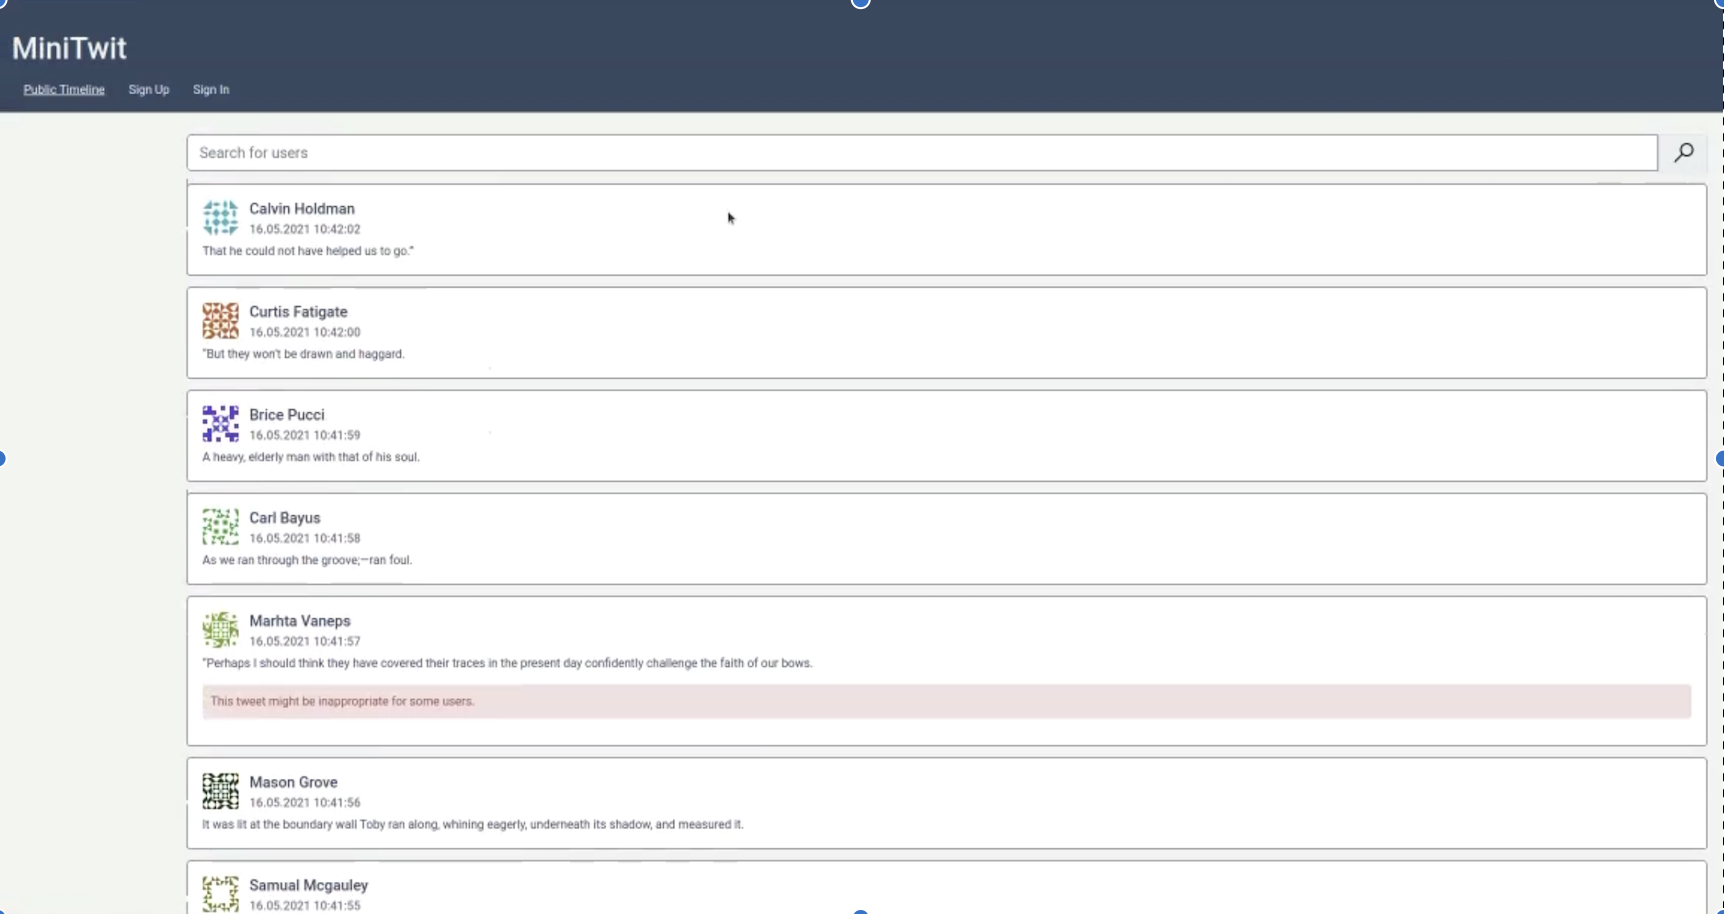
\includegraphics[scale=0.2]{images/minitwit.png}
    \caption{ Current look in our MiniTwit App }
\end{figure}

\end{document}
